\documentclass{article}
% main document, called main.tex
\usepackage{tikz}
\usetikzlibrary{external}

\usetikzlibrary{positioning}
\usetikzlibrary{calc}
\usetikzlibrary{shapes.geometric, arrows, arrows.meta}
\usepackage{varwidth}% http://ctan.org/pkg/varwidth
\usetikzlibrary{shadows,trees, mindmap}
\usetikzlibrary{matrix}
\usetikzlibrary{fit}

\tikzexternalize % activate!
\begin{document}

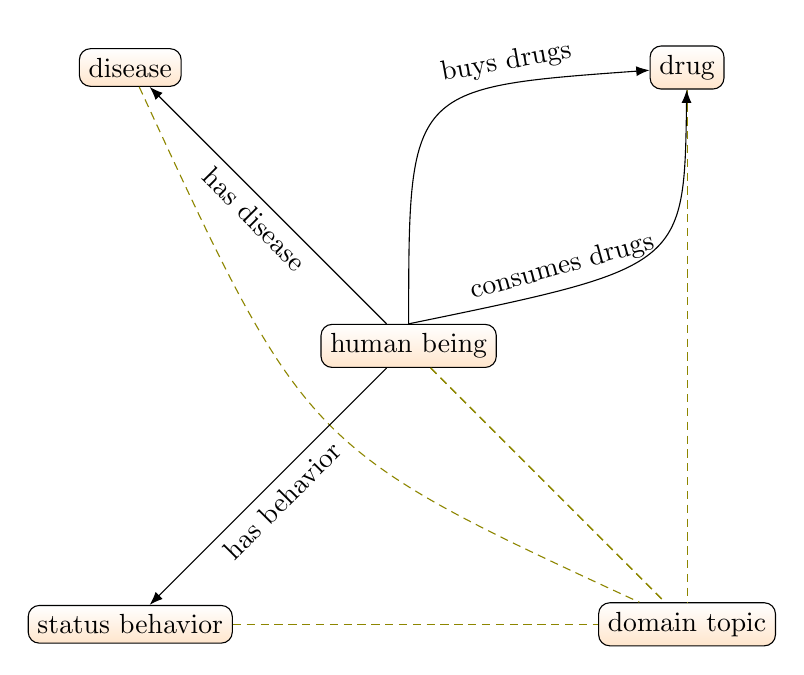
\begin{tikzpicture}[
concept/.style={shape=rectangle, rounded corners,
draw, align=center,
top color=white, bottom color=orange!20},
node distance=5cm,
]
\node [concept] (human) {human being};
\node [concept, below right of=human] (domain) {domain topic};
\node [concept, above left of=human] (disease) {disease};
\node [concept, below left of=human] (status) {status behavior};
\node [concept, above right of=human] (drug) {drug};

\draw[densely dashed, color=olive] (human) -- (domain);
\draw[densely dashed, color=olive] (disease) .. controls ($(human) + (-1.3cm,
		-1.3cm)$) .. (domain); 
\draw[densely dashed, color=olive] (status) -- (domain); 
\draw[densely dashed, color=olive] (drug) -- (domain); 
\draw[densely dashed, color=olive] (human) -- (domain); 

\draw [-Latex] (human.north) .. controls ($(human.north) + (0cm,
3cm)$) ..  (drug) node [sloped, above, near end] {buys drugs}; 
\draw [-Latex] (human.north) .. controls ($(human) + (3.5cm, 1cm)$)
..  (drug) node [sloped, above, near start] {consumes drugs}; 
\draw [-Latex] (human) -- (status) node [below, midway, sloped] {has behavior}; 
\draw [-Latex] (human) -- (disease) node [below, midway, sloped] {has disease}; 

\end{tikzpicture}


\end{document}




